% The Chuzhditsa typeface — concise implementation description (XeLaTeX; fonts in ../fonts/)
% The construction history this paper no longer narrates lives in the repository's
% git log and in the companion process paper.
\documentclass[12pt]{article}
\usepackage[a4paper,margin=2.7cm]{geometry}
\usepackage{fontspec}
\usepackage{booktabs}
\usepackage{graphicx}
\usepackage[font=small,labelfont=bf]{caption}
\usepackage{microtype}
\usepackage{setspace}
\usepackage{amsmath}
\setlength{\emergencystretch}{2em}
\usepackage[hidelinks]{hyperref}

\setmainfont{Times New Roman}
\newfontfamily\ipafont{Arial Unicode MS}[Scale=MatchLowercase]
\newfontfamily\chu[
  Path = ../fonts/v3/ ,
  Extension = .ttf ,
  UprightFont = ChuzhditsaInline-Regular ,
  BoldFont = ChuzhditsaInline-Bold ,
  ItalicFont = ChuzhditsaInline-Italic ,
  BoldItalicFont = ChuzhditsaInline-BoldItalic ,
  ]{ChuzhditsaInline-Regular}
\newcommand{\cz}[1]{{\chu #1}}
\newcommand{\ph}[1]{{\ipafont/#1/}}

\title{\textbf{The letter as a program:\\ how the Chuzhditsa typeface works}}
\author{{\normalsize [ANON]}\thanks{The builder discussed here ($\sim$800 lines of Python) is distributed with the fonts in an open repository ([ANON] — redacted for review); every object-language example in this manuscript is set in the typeface under discussion. A companion system paper ([ANON]) documents the orthography this family serves.}}
\date{}

\begin{document}
\special{pdf:docinfo << /Title (The letter as a program: how the Chuzhditsa typeface works) >>}
\maketitle
\onehalfspacing

\begin{abstract}
\noindent Chuzhditsa is a Cyrillic typeface family of four cuts — a round-capped register face, a grotesk, a slab serif, and an inline cut weight-matched to Times for setting citations inside serif text — each in Regular, Bold, Italic, and Bold Italic, generated entirely from one set of centerline skeletons by a parametric builder of roughly eight hundred lines. The family exists to serve a designed writing system: a phonological citation register that extends Cyrillic for writing foreign words so that their source pronunciation is recoverable. This paper describes how the typeface works, as an implementation. A stroke model declares every glyph as centerline primitives and expands them with a disc whose diameter varies with the path's tangent angle, supplying both page texture and junction relief in one function. A boolean-union outline policy resolves at build time what coverage-summing and even-odd rasterizers would otherwise mishandle. An optical-correction canon — overshoots, apex piercing, optical centering, round compression — is implemented as build-time arithmetic, with every coordinate derived from a single parameter sheet. Per-family terminal, slab, and clamp rules separate the four cuts; a six-class kerning matrix covers the fitting space in thirty rules that extension letters inherit by construction. The OpenType layer functions as an executable reference implementation of the orthography the face serves: ligature lookup order, register-gated fusions, computed mark anchors, and a normalization-closed character map, verified by a shaping-test suite. An instrumented evaluation measures per-cut small-size floors, and the build is byte-reproducible. The parametric claim is deliberately scoped: parameters hold within one design language, never across all letterforms.

\medskip
\noindent\textbf{Keywords:} Cyrillic; OpenType; optical corrections; parametric type design; type engineering; writing systems

\medskip
\noindent\textbf{Implications for practice.} The transferable content is a set of named rules with stated rationales: union overlapping outlines before emitting, because coverage-summing rasterizers darken every seam and even-odd consumers open white slits; ship pair kerning as GPOS, because the legacy kern table is ignored in CFF-flavored fonts; widen advances with weight, because advance width is a property of the counter, not the stroke; trim advances on open-sided letters, whose apertures recede; and derive every coordinate from the parameter sheet, so that a value which holds in only one style is exposed as a bug rather than shipped as a glyph. Treating optical corrections as engine-level arithmetic lets them generalize across a large character set at no marginal cost. For designers extending scripts for new orthographies, the executable-reference-implementation pattern — spelling rules compiled as OpenType lookups and verified by shaping assertions — makes orthographic claims mechanically testable.
\end{abstract}

\section{Introduction}

A companion paper ([ANON]) describes Chuzhditsa's function: a \emph{phonological citation register} for pan-Slavic Cyrillic — a system for writing foreign words, names, and pedagogical examples so a Cyrillic reader can recover the source pronunciation — whose extension letters are derived by a small set of recurrent diacritic operations. A writing system whose \emph{letters} are rule-derived invites a typeface whose \emph{glyphs} are rule-derived: the two grammars mirror each other, and several orthographic rules (ligature fusion, mark anchoring) exist in the font as executable code rather than prose. This paper describes that implementation. Given a designed orthographic register — this one or another — the question answered here is what it takes to make it typographically real.

The parametric commitment is total, and ``the construction is the design'' reduces to checkable properties: (i) there is no drawn master anywhere in the pipeline — the skeleton declarations and the engine are the only sources; (ii) one specification generates both the shapes and the OpenType behavior; (iii) the optical-correction canon is encoded at the engine level, not applied per glyph; and (iv) the font operates as a conformance implementation for a designed writing system, with shaping tests as its test suite. The claim is scoped from the outset: Knuth's proposal that a typeface can be a program (Knuth, 1982) fails, as Hofstadter (1982) argued, for \emph{all} letterforms — and succeeds for one design language at a time. Within a single stroke grammar, weight, slant, contrast, terminal finish, and vertical scale genuinely are parameters, and the family's sixteen styles are evaluations, not drawings; this is also the position variable-font practice reached by another road, interpolating within one design space and claiming nothing beyond it.

Five terms carry precise senses in what follows. The \emph{orthography} is the mapping from phonological input to character sequences; the \emph{register} is the functional category being marked (foreign-word citation); the \emph{typeface} is the design language; the \emph{font binary} is the executable artifact — glyphs, cmap, GSUB/GPOS, anchors; and the \emph{text encoding} is the Unicode character sequence, which preserves the orthography's letters in plain text but preserves the register only where font control survives.

\begin{figure}[ht]\centering
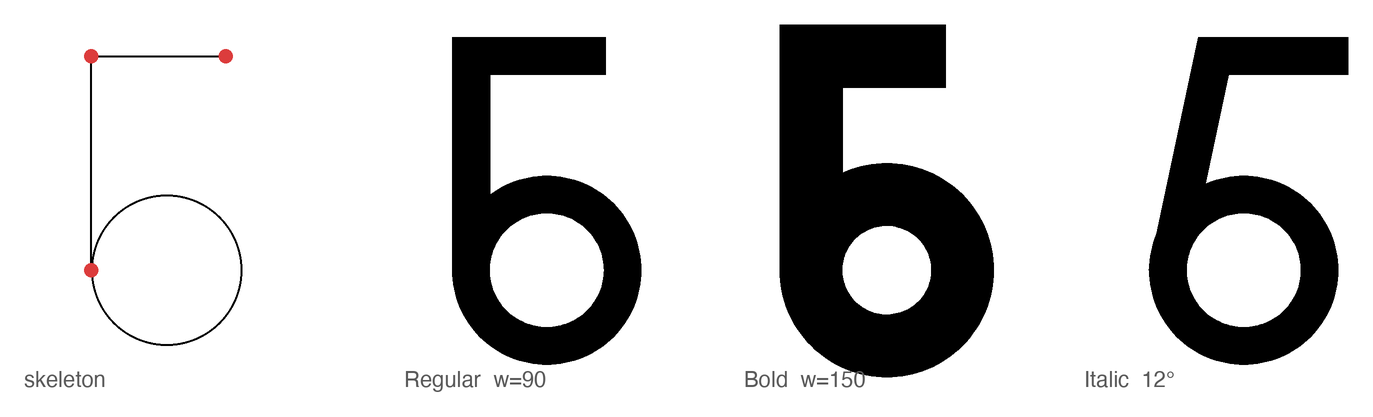
\includegraphics[width=1.00\linewidth]{figures/fig1_stroke_model.png}
\caption{The stroke model. Left: the declared skeleton of \cz{Б} — two line strokes and a bowl arc whose endpoints (marked) terminate in the stem, the anatomy every reference Cyrillic face uses for the D-countered bowls. Right: the same declaration evaluated at two weights and a 12° slant. Nothing between the panels was drawn.}\label{fig:stroke}
\end{figure}

\section{The stroke model}

Noordzij's theory holds that the letter is built of strokes, each the trace of a frontline segment — Noordzij's \emph{front} — advancing along a path (Noordzij, 2005). Chuzhditsa is that theory made executable in a near-monoline case. Every glyph is declared as centerline primitives — straight segments, circular arcs, full rings, dots — in a 1000-unit em (Figure~\ref{fig:stroke}). The entire artwork of a letter is a line of Python; here is a bowl-and-stem letter, in full:

{\small\begin{verbatim}
"b": dict(adv=660, strokes=[(R,340,190,180),      # ring: bowl
                            (L,160,190,160,700),  # line: stem
                            (L,160,700,480,700)]) # line: top arm
\end{verbatim}}

\noindent The engine expands each path by sweeping a disc along it, with the disc's diameter a function of the path's tangent angle:
\[ w(\theta) \;=\; w_h + (w_v - w_h)\,\lvert\sin\theta\rvert^{1.3}, \]
so verticals carry the full stem weight $w_v$, horizontals the family's contrast fraction of it, and diagonals and arcs interpolate; on a ring the modulation lands exactly where broad-pen contrast would. The exponent and the per-family contrast values are parameters (Table~\ref{tab:params}). Besides supplying texture, the function solves junction density without a dedicated rule: where several strokes converge (\cz{ж} center, \cz{д} crossbar, \cz{ѫ} fork), the converging strokes are non-vertical, so the thinning arrives precisely where ink would otherwise double.

The italic applies its shear \emph{to the centerlines before expansion}, not to the finished outlines: a sheared outline modulates its own thickness (the singular values of a 12° shear are about 0.90 and 1.11, a visible $\pm$10\% wobble around a ring), whereas a sheared centerline swept by an unsheared disc keeps constant perpendicular weight — the trace of a \emph{round} nib, whose width does not vary with direction (Figure~\ref{fig:italic}). This is precisely not Johnston's broad-edged pen (Johnston, 1906), whose defining behavior is width that varies with direction; the round-nib model is the right one here exactly because the face has almost none of the broad pen's contrast. Because the contrast function operates on post-shear tangents, contrast and slant compose.

\begin{figure}[ht]\centering
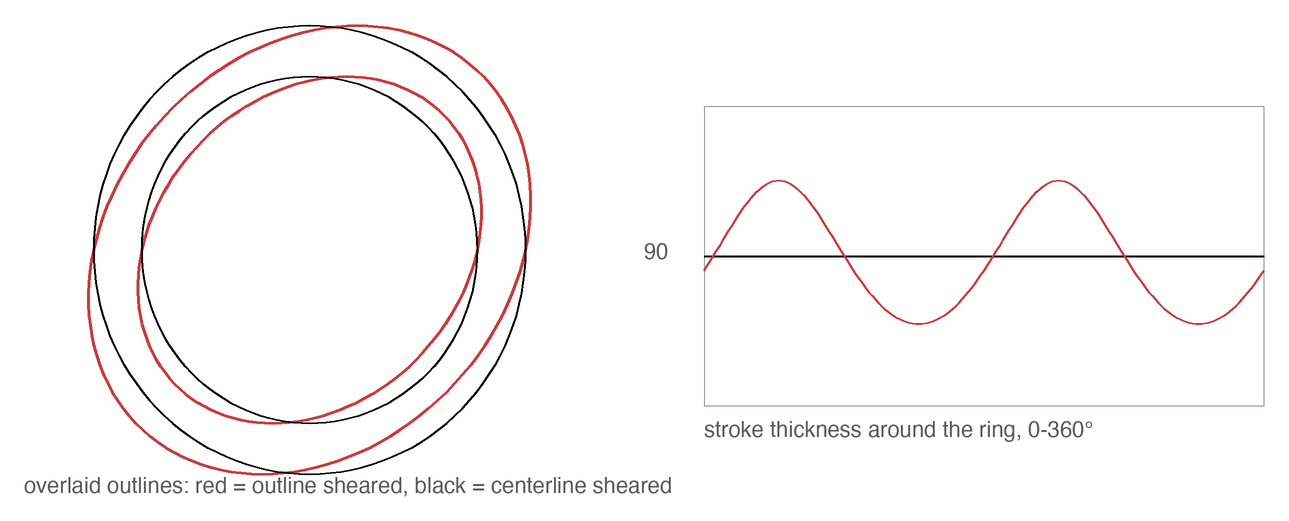
\includegraphics[width=1.00\linewidth]{figures/fig6_italic.png}
\caption{Two ways to make an italic \cz{О}. Left: shearing the finished outline modulates the ring's own thickness. Right: shearing the centerline and sweeping an unsheared disc preserves constant perpendicular weight.}\label{fig:italic}
\end{figure}

Expansion emits per-segment quadrilaterals with end discs, densely sampled (arcs at one point per 2.5°, circles at 48--128 points by radius; no Bézier segments), and then \textbf{boolean-unions every glyph into disjoint, consistently wound outlines before emitting}. The union is not cosmetic. Overlapping contours are rendered correctly by nonzero-winding rasterizers, but rasterizers that sum antialiasing coverage per contour darken every overlap seam — a face built of overlapping quads and discs reads as a smeared pseudo-bold in such viewers — and even-odd consumers (a naive SVG export, some diagnostic renderers) open white slits at folds and cancellations. Union settles every case at build time, and incidentally keeps the binaries small (60--100\,KB per style for 184 codepoints). The rule for the next implementer: orient before you overlap, or union before you emit.

The small primitive vocabulary is deliberate, because every primitive is a maintenance contract. A ring is not ``a circle the designer drew'' but a promise that bowls respond as a class to any future correction: one clamp repairs every bowl in the family at once; one factor narrows every full round. In an extension set serving thirty-plus orthographies, corrections that do not generalize do not get made — the economics Bigelow and Holmes reported from the first large Unicode face, where coherence at character-set scale is the product of harmonization rather than glyph-by-glyph invention (Bigelow \& Holmes, 1993). Monoline construction is easy to mistake for the easy case; it is the opposite. Contrast hides sins: where a modulated face can thin a stroke through a crowded joint, a near-monoline must resolve every collision honestly, in geometry. The rules of \S\ref{sec:rules} are those resolutions.

\section{Design constraints}

The visual register must be recognizably \emph{other} at reading distance while remaining effortlessly legible to any Cyrillic reader — the katakana condition. The letterforms therefore keep utterly conventional Cyrillic skeletons — Zhukov's account of what makes Cyrillic Cyrillic (the correlated treatment of \cz{А Л Д М}, of \cz{Б В Р Ч Ъ Ы Ь Я}, the dominance of verticals and straight-line construction in the lower case) was treated as a constraint list (Zhukov, 1996) — while the \emph{style} carries the register: full-circle bowls in the manner of round Glagolitic, whose loops survive in \cz{б в р ъ ь ы ю}, and one construction vocabulary shared by both cases. For a Bulgarian-born project the styling also takes a documented side in Bulgarian typography's own letterform discourse — heritage forms for heritage letters (Yonchev \& Yoncheva, 1982).

Designing against the whole Slavic superset disciplines individual letters in ways single-language design would not. The clearest case: a wide, round \cz{е} — the historic ``broad e'' — turns out to be the shape of Ukrainian \cz{є} (U+0404), a distinct letter with its own phonemic identity, so \cz{е} takes a closed bowl (aperture roughly half the open forms') and \cz{є} keeps the wide aperture and a half-bar; the contrast survives by shape, not bar length alone. The general rule: in a multi-orthography script the letterform space is commons, and a design that grazes it for one language will silently fence off a neighbor's letter. Design against the superset first.

\section{Letterform rules}\label{sec:rules}

\subsection{Terminals, slabs, and clamps}
Terminal finish is a family parameter, not a per-glyph decision. The 2b register face carries round caps — affordable because the tangent-angle taper already modulates the stroke; a strictly uniform stroke reads them as marker pen. The Grotesk drops the end disc at every \emph{free} terminal: one whose endpoint does not lie within 32 units of another stroke's endpoint — an endpoint-sharing test, since shared joints keep their discs and the disc is what fills the joint. The Serif and Inline grow slabs by a placement-plus-suppression rule: slabs grow only on near-vertical line terminals ($\lvert\sin\theta\rvert \ge 0.93$) whose endpoints sit at the guide lines, and are suppressed where the terminal is shared with another stroke or already covered by a crossbar — stems take feet at the baseline, and nothing sprouts where a bar already closes the form.

Counters are protected by clamping stroke weight against curvature: a closed bowl of radius $r$ carries at most $0.85r$ of stroke, an open arc at most $r$ (an open arc keeps half its radius of daylight, so it can afford the extra weight). The clamp earns its keep at the small end of the range — a Bold breve is an arc of radius 130 asked to carry a 150-unit stroke, more ink than circle — and is the programmatic form of the punchcutter's counter-first discipline (Smeijers, 1996): the stroke narrows to what the curve can hold, and nobody notices, which is the intended outcome (Figure~\ref{fig:clamp}). A second, declaration-level clamp handles the letters whose \emph{diagonals} clog: the skeletons tag the legs of \cz{ж х} as a distinct stroke kind, and only those segments are clamped (Serif to 108 units, Inline to 86), so \cz{у}'s plain diagonals escape by design.

\begin{figure}[ht]\centering
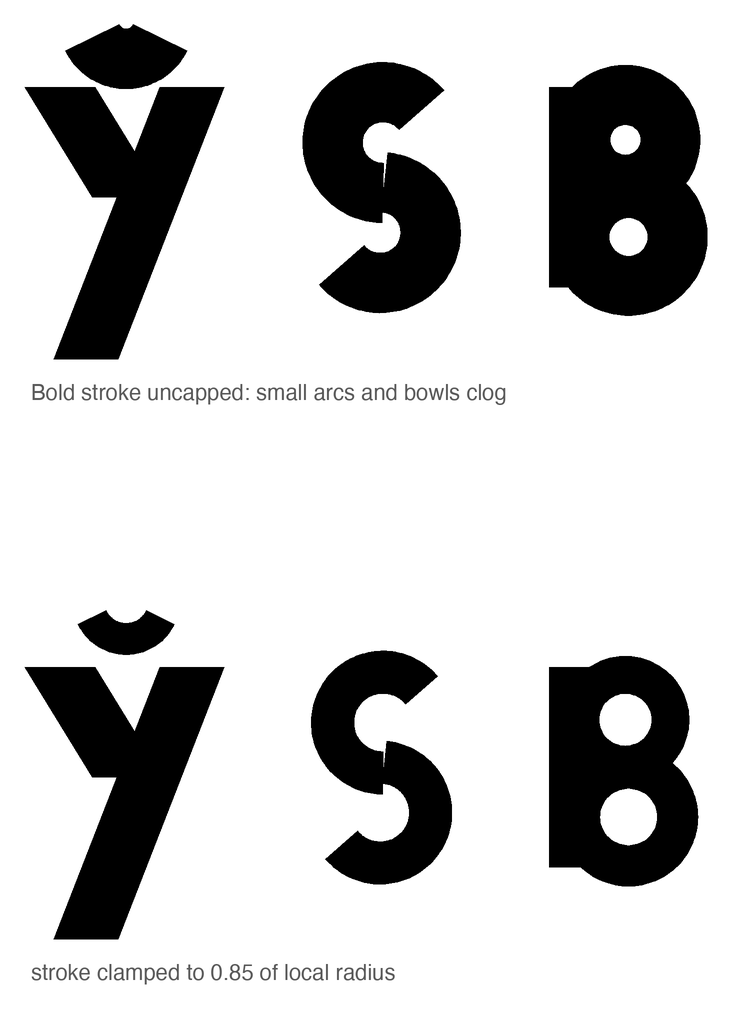
\includegraphics[width=0.60\linewidth]{figures/fig14_clamp.png}
\caption{Curvature-clamped weight. Above: Bold's full stroke applied to the breve of \cz{ў} and the bowls of \cz{ѕ в} clogs them shut. Below: stroke clamped to the local radius budget ($0.85r$ closed, $r$ open) — the counters breathe, the weight reads unchanged.}\label{fig:clamp}
\end{figure}

Bold is not thick Regular: with a heavier stroke in slots spaced for the lighter one, every pair loses air and the fitting collapses \emph{unevenly} — first where air was scarcest, so a bold \cz{о} welds into a following \cz{л} while straight-sided pairs merely tighten. The Bold therefore buys back its ink: advances widen with the weight ($+$12 units of sidebearing and a 1.10 frame scale), and each glyph re-centers (Figure~\ref{fig:bold}). The rule of thumb: \emph{in a parametric near-monoline, weight is a property of the page color, but advance width is a property of the counter.}

\begin{figure}[ht]\centering
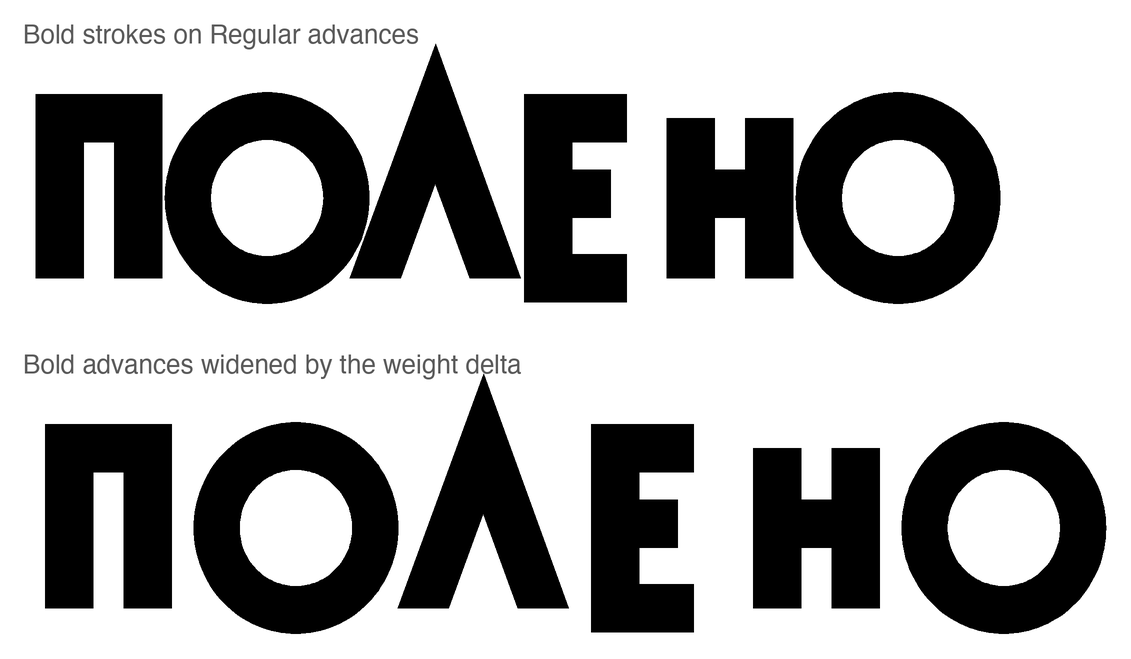
\includegraphics[width=0.93\linewidth]{figures/fig5_bold_color.png}
\caption{The same word, Bold strokes. Above: on Regular advances the fitting collapses unevenly — \cz{о} welds into \cz{л} while pairs with air to spare merely tighten. Below: advances widened with the weight and glyphs re-centered — the fitting, and the counters, survive.}\label{fig:bold}
\end{figure}

\subsection{The optical canon, computed}
Every ``geometric'' face is a catalogue of concealed corrections — Renner's Futura most famously (Burke, 1998, pp.\ 101--102). Chuzhditsa implements the canon as build-time arithmetic:

\begin{itemize}
\item \textbf{Overshoot of rounds.} Flat letters read taller than round ones of equal height, so full rounds overshoot the cap band and undershoot the baseline. Overshoot is measured against the \emph{rendered envelope} of rounded terminals — half a stroke past the guides — not against the guides, and it is a function of curve breadth and weight, not a constant: a broad bowl takes $+$48 units of vertical radius, while the narrow bowls of \cz{а р} take $+$32 at text weights, because at equal ink height a narrow bowl reads taller — the ellipse concentrates its extreme into a smaller arc. The Bold keeps the full value; its wider stroke flattens the extreme back out.
\item \textbf{Overshoot of apexes.} A point that stops exactly at the cap line reads short — the eye averages the vanishing wedge. The apexes of \cz{А Л Д Ѫ Ѧ} pierce the line by 15--18 units; their feet, conversely, sit flat — a point may pierce a line it approaches; a letter should not balance on one.
\item \textbf{Optical center.} A crossbar at the geometric middle appears to sag; the bars of \cz{Е Н} sit above geometric centre — the lettering classroom's rule that the apparent centre lies ``very slightly above mid-height'' (Johnston, 1906, pp.\ 273--274). Bar \emph{length} on open-sided letters is likewise derived, not fixed: the bar of \cz{е є Е} terminates at $r\cos(0.75\,a)$ for aperture $a$, flush with the arc tips at any aperture and any weight — a fixed fraction of the radius outruns the aperture's arc tips and reads as a spike.
\item \textbf{The circle that is not.} A mathematically perfect circle beside rectangular letters reads wide; all full-height rounds are compressed 3.5\% horizontally. The correction is invisible, which is the point (Bringhurst, 2004, p.\ 17).
\end{itemize}

Joints between arcs and bars sit \emph{on the live radii} — a connection point is $(c_x + r_x\cos\vartheta,\; c_y + r_y\sin\vartheta)$ of the current style's radii, never a copied coordinate — which is an instance of the engine's governing discipline: \emph{every coordinate is either derived from the parameter sheet or it is a style bug that has not yet found its style.} Figure~\ref{fig:optical} shows the canon one variable at a time; none of the numbers is proposed as a universal constant — all were set by proofing and are published as the reproducible record of one face's optical parameters. What deserves emphasis is how small the winning corrections are: 2.5--3.5\% each, individually invisible at reading sizes, and collectively the entire difference between a naïvely expanded stroke font and a credible one. The eye audits at a precision it does not report.

\begin{figure}[ht]\centering
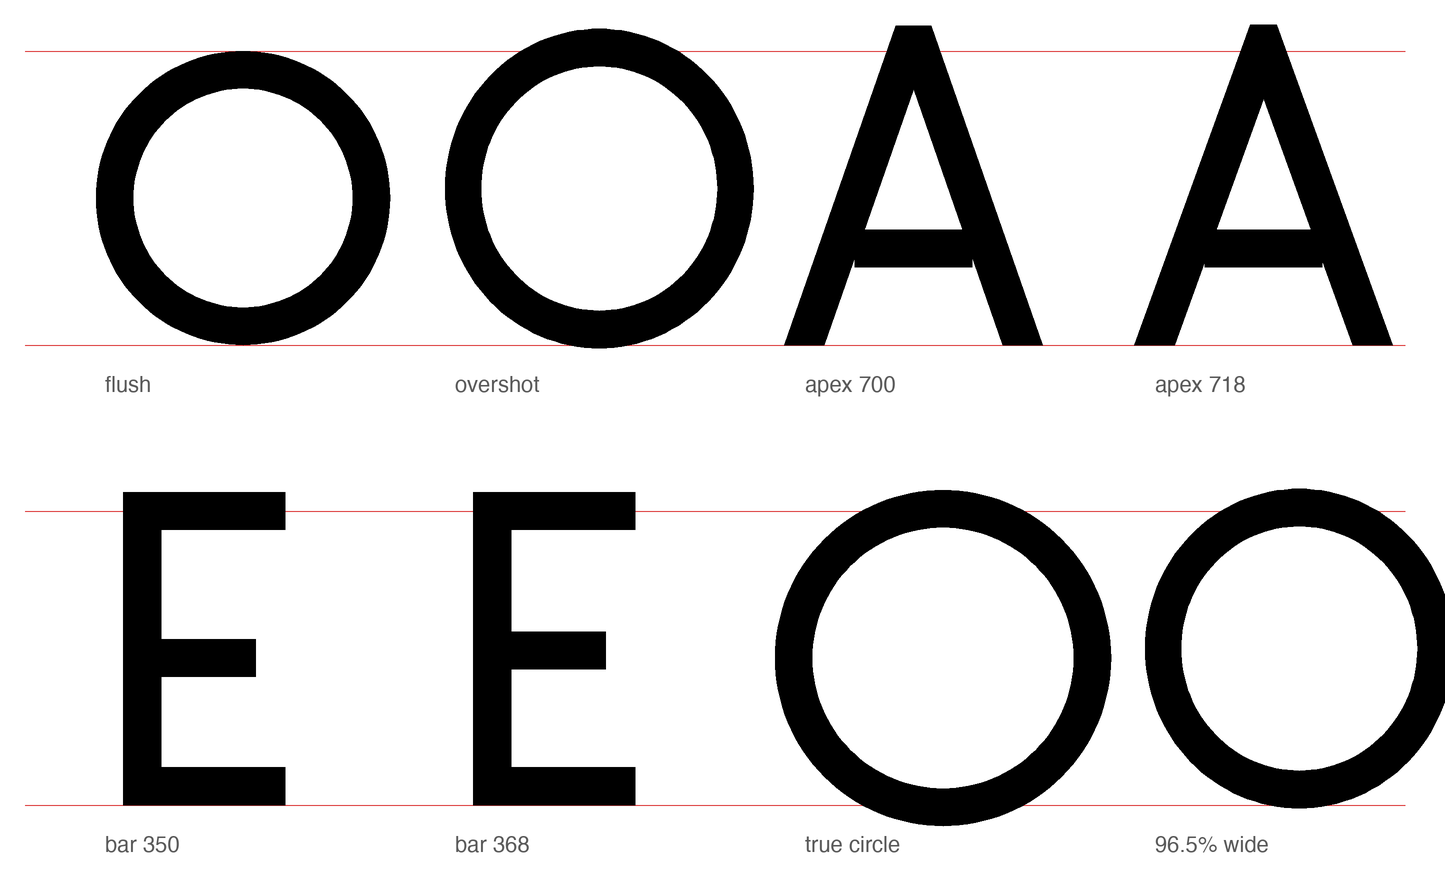
\includegraphics[width=1.00\linewidth]{figures/fig4_optical.png}
\caption{The optical canon, one variable at a time, on ruled cap and base lines. Flush versus overshot rounds; apex at the cap line versus pierced through it; crossbar at the geometric versus optical center (shown on a schematic block \cz{Е}, not the shipped round form); a true circle versus the shipped 96.5\% width.}\label{fig:optical}
\end{figure}

For the record — and because a parametric face can state its entire design in one table where a drawn face cannot — Table~\ref{tab:params} is the complete parameter sheet.

\begin{table}[ht]\centering\footnotesize\setlength{\tabcolsep}{2pt}
\begin{tabular}{llll}
\toprule
Parameter & Value & Parameter & Value \\
\midrule
em / cap / x-height & 1000 / 700 / 500 (design grid) & apex overshoot & +15--18 \\
contrast function & $w_h=0.90\,w_v$ base, exp.\ 1.3 & full-bowl overshoot & $+$48 vertical radius \\
2b text master & stems 76 / 122; sb $+$8 & narrow-bowl overshoot & $+$32 (\cz{а р}, text) \\
grotesk & 84, contrast 0.08, butt & optical bar rise & above centre (\cz{Е Н}) \\
serif & 92, contrast 0.34, slabs & round compression & 96.5\% (radius $\geq$ 200) \\
inline cut & stems 80, contrast 0.54 & weight clamp & ring $0.85r$; open arc $r$ \\
inline scaling & yScale 0.88, caps 1.071, frame 0.93 & diagonal clamp & serif 108 / inline 86 (\cz{ж х}) \\
inline slabs & 52$\times$16, thin-stem & aperture & 55° 2b, 50--52° rest; \cz{е} closed \\
italic slant & 10° (centerline, post-shear tangents) & bar terminus & arc tips: $r\cos(0.75\,a)$ \\
Bold advance rule & $+$12 sb, frame $\times$1.10 & curve joints & on live radii $(r_x\cos\vartheta, r_y\sin\vartheta)$ \\
kern matrix & 6 classes, 30 rules, $-$4 \ldots $-$95 & Bold kern scale & $\times$0.7 ($\times$1.3 top-bar) \\
compiled kern pairs & $\sim$15{,}000 / style & curve sampling & 48--128 pts by radius; arcs 2.5°/pt \\
grotesk butt test & free terminal: no endpoint within 32 & slab rule & $\lvert\sin\theta\rvert{\ge}0.93$, at guides, unshared \\
\bottomrule
\end{tabular}
\caption{The complete parameter sheet of the v3 family builder. Every visual property of the four families derives from this table plus the per-glyph skeleton declarations.}
\label{tab:params}
\end{table}

\section{Four cuts from one skeleton}\label{sec:cuts}

Cap finish, slabs, contrast, clamps, and vertical scale are \emph{family} parameters of the one engine: the four faces share every skeleton and the whole kerning matrix, separated only by their parameter sheets (Figure~\ref{fig:specimen}).

\begin{itemize}
\item \textbf{2b} — the register face: round caps, contrast 0.10, the archaic round-bowl styling at full strength.
\item \textbf{Grotesk} — butt terminals, contrast 0.08: a screen and UI alternate. 2b and Grotesk share every proportion and part mainly at the terminal, so the honest count is two well-separated cuts (Serif, Inline) and one register face with a grotesk alternate; the point is the parameter mechanism, not four unrelated designs.
\item \textbf{Serif} — slab feet, contrast 0.34, the diagonal clamp at 108: a longer-form reading cut.
\item \textbf{Inline} — the citation cut, for register words set inside a serif page (the name marks the \emph{use}, set inline in running text, not the engravers' incised-stroke sense). It is scaled to serif proportions — x-height $\times$0.88, frame $\times$0.93, capitals $\times$1.071 (Cyrillic's x-to-cap ratio is taller than Times', so no single vertical scale can match both) — with stems 80 at contrast 0.54 and thin-stem slabs 52$\times$16. The weight was matched to its host by reader proofing rather than density metric, and landed at roughly 95 percent of Times' own stem weight with the fit slightly open: evenly weighted geometric forms read darker than modulated serif forms at equal measure, so perceived color match is not mean-ink match. This manuscript's object language is set in it.
\end{itemize}

The family is fully two-case. Capitals derive from the lowercase skeletons ($\times$1.10 horizontal, $\times$1.4 vertical); the capitals whose anatomy is not a scaling — \cz{А Б Д Е О С У Ф Я Һ} and kin — carry their own constructions (Figure~\ref{fig:cases}). Within the lowercase, \cz{һ} is the set's one ascender and \cz{р ф д} its descenders; the capital \cz{Һ} keeps the lowercase hoop unchanged beneath a cap-height stem, the anatomy of the reference faces.

\begin{figure}[ht]\centering
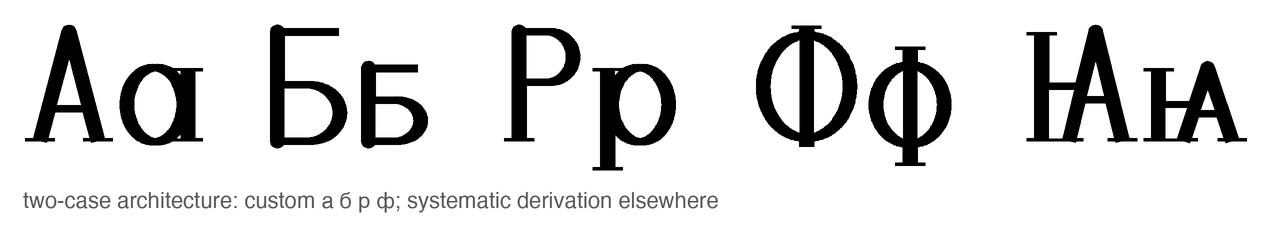
\includegraphics[width=1.00\linewidth]{figures/fig10_cases.png}
\caption{Case pairs. Capitals derive from the lowercase skeletons where anatomy permits; letters whose capital form is not a scaling carry their own constructions.}\label{fig:cases}
\end{figure}

\begin{figure}[ht]\centering
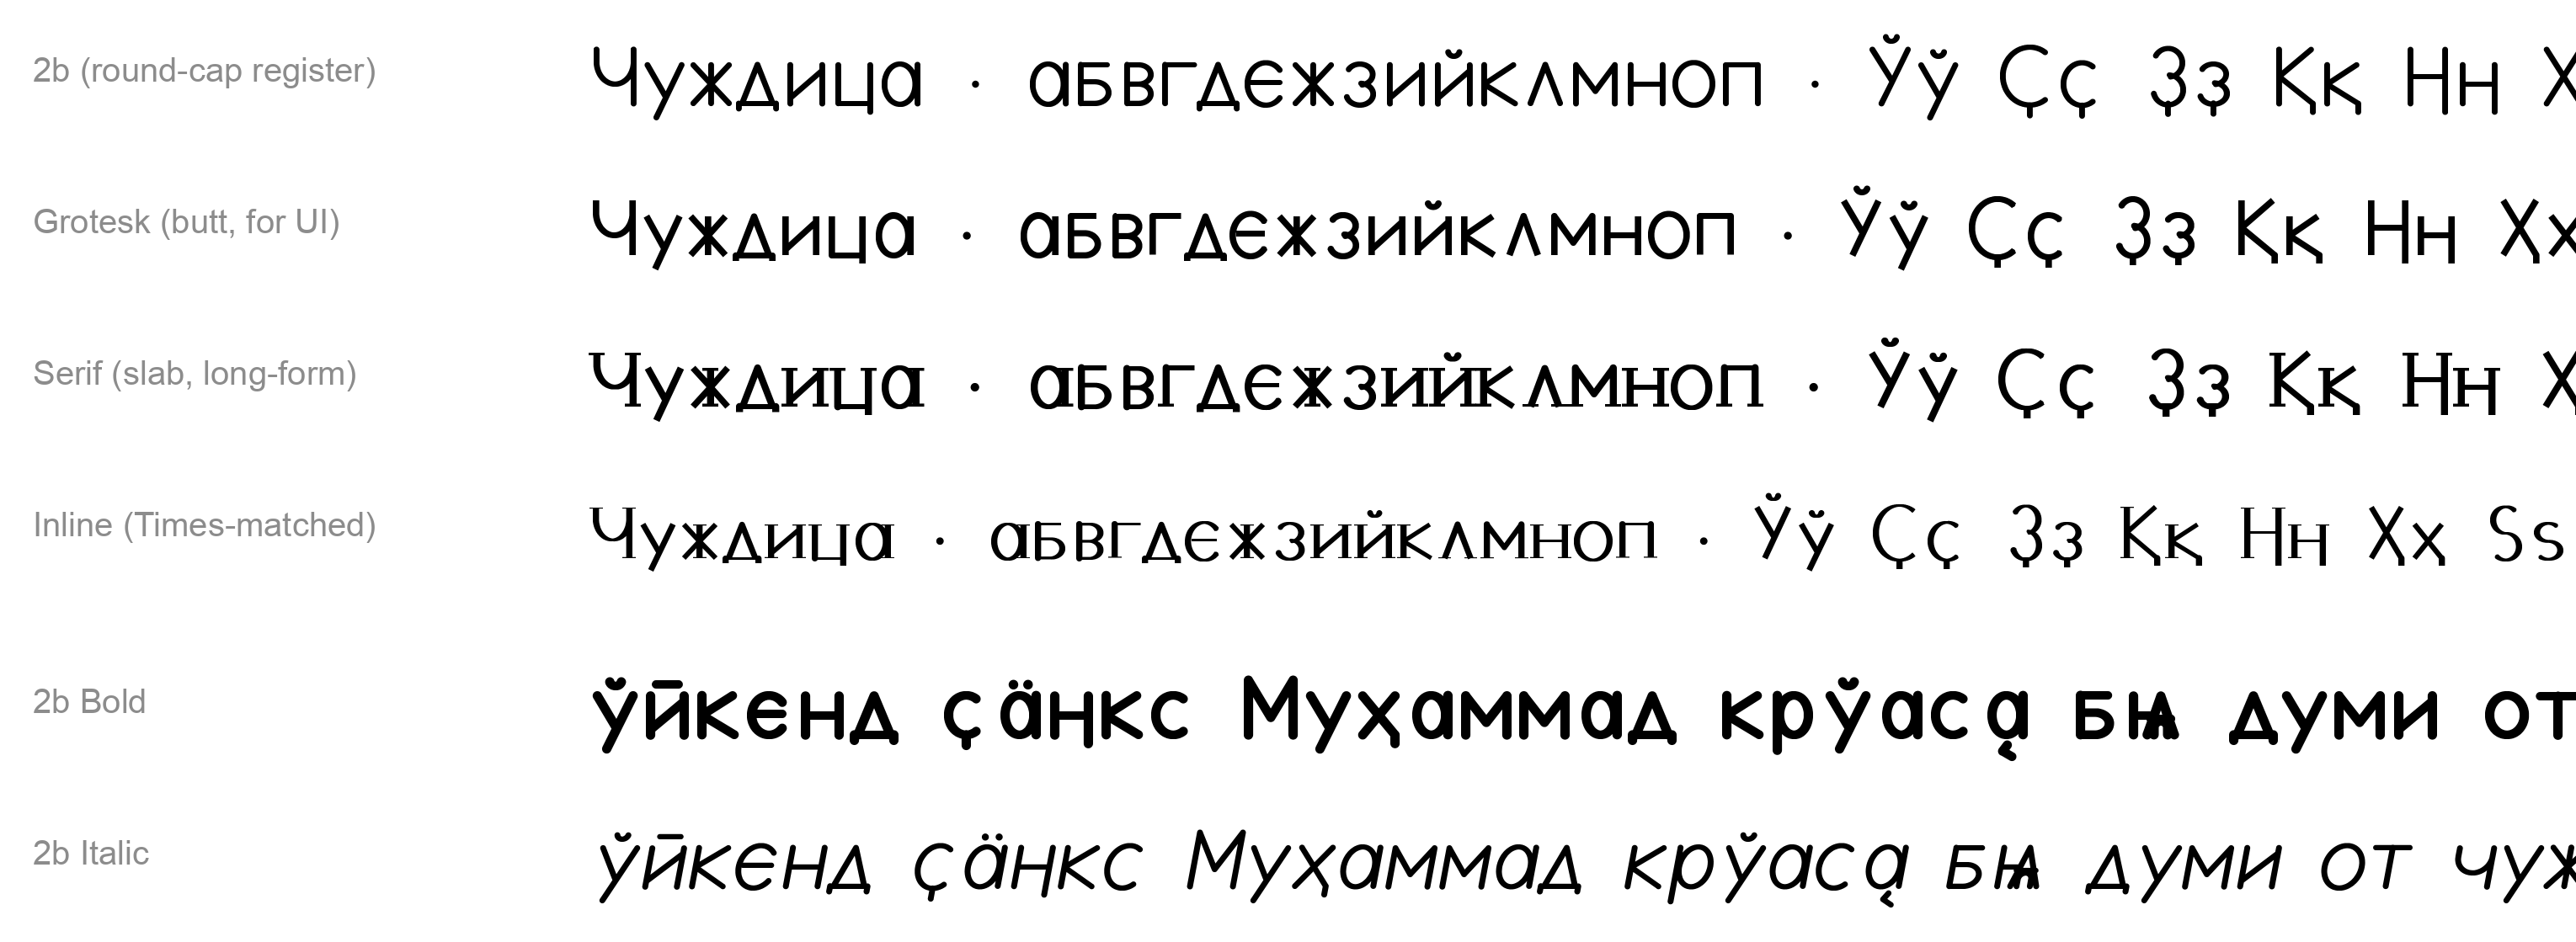
\includegraphics[width=0.99\linewidth]{figures/fig9_specimen.png}
\caption{The four families from one skeleton set — 2b (round-cap register), Grotesk (butt, alternate to 2b), Serif (slabs), and Inline (weight-matched to Times for citation inside a serif page) — above the 2b Bold and Italic. Every family carries the full extension inventory, the register cuts additionally the ligature fusions; all panels are set from the shipped binaries through the deployment shaping stack.}\label{fig:specimen}
\end{figure}

\section{Fitting and kerning}\label{sec:fitting}

Fitting is per-glyph advances under a per-family scalar sidebearing. The advances encode a rule the aperture letters make vivid: \emph{an open side is not a round side}. The letters that open rightward or leftward (\cz{с ҫ б з э} and the capitals \cz{С Ҫ}) take advances trimmed well below their round siblings', because the aperture recedes and the default round-letter advance leaves a hole the eye reads as a word break; the same logic trims the top-bar letters' left approach. Tracy's dictum that fitting is fundamental to a design's success (Tracy, 1986, p.\ 71) survives translation into a parametric setting with interest: roughly half of this face's perceived quality lives in decisions about white (Figure~\ref{fig:fitting}).

Kerning is class-based and shallow by design. Every glyph is assigned a left and a right \emph{side class} from a six-class vocabulary — round, flat, diagonal, top-bar (the overhanging arms of \cz{т г}), apex (\cz{д л ѫ А}, whose top-centre point leaves a void under a preceding arm), and aperture (the open sides of \cz{с ҫ з}, whose facing voids compound) — and thirty pair rules cover the space, from flat$\times$flat 0 to top-bar$\times$apex $-$95. Extension letters inherit their base letters' side classes by construction — \cz{ғ ѓ} kern as \cz{г}, \cz{ў} as \cz{у}, \cz{ӓ} as \cz{а} — so the extension inventory inherits fitting for free. Compiled over the full 184-codepoint coverage, the matrix expands to $\sim$15{,}000 nonzero pairs per style. Bold scales the rhythm kerns to $\times$0.7 of Regular — its thicker strokes close the same gaps optically — but \emph{boosts} the structural top-bar kerns $\times$1.3: the void under an overhanging arm is geometry, not rhythm, and it grows with the Bold's wider frame. Deep pair lists are where parametric discipline goes to die, since every hand-set pair is an exception to the system; where a class rule cannot fix a combination, the collision is treated as evidence about a \emph{glyph} — usually an advance wrong on one side — and the letter is repaired, not the pair.

\begin{figure}[ht]\centering
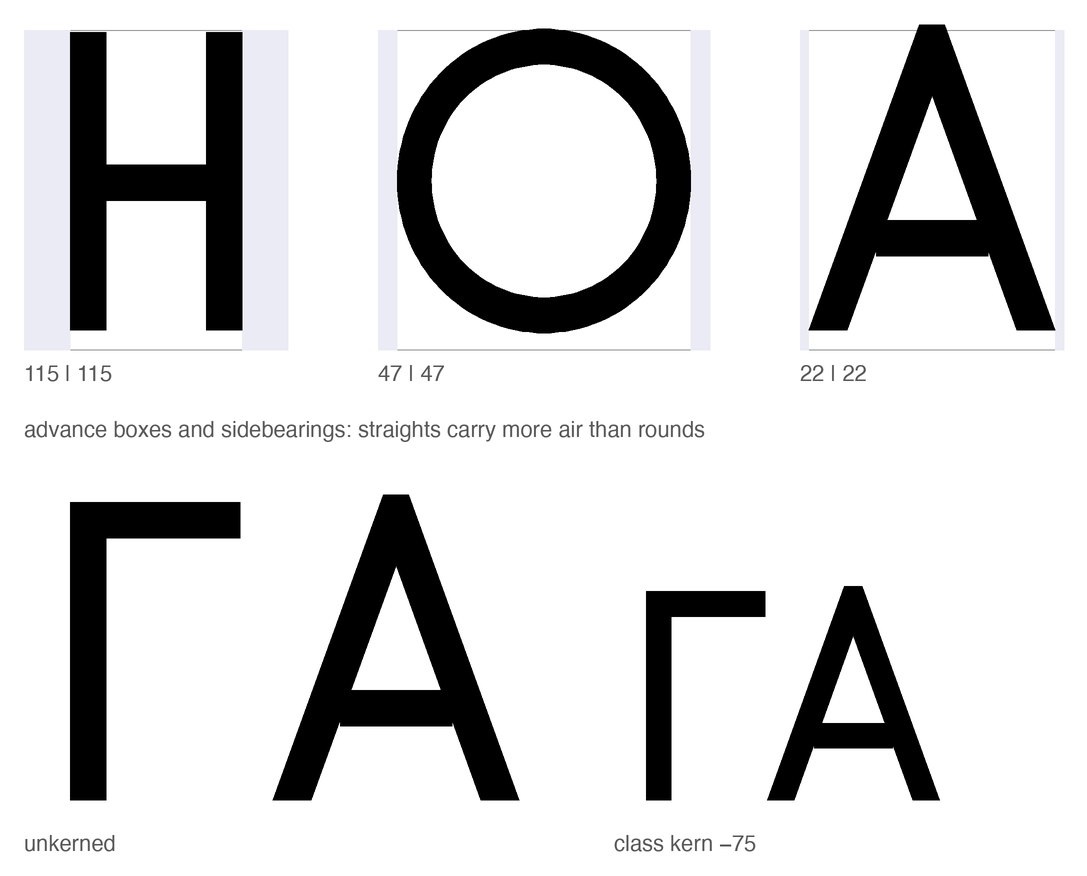
\includegraphics[width=0.88\linewidth]{figures/fig15_fitting.png}
\caption{Fitting. Left: advance boxes and sidebearings for a straight, a round, and a diagonal letter — the intended hierarchy of white. Right: a top-bar-over-apex pair at raw advances and under its class kern.}\label{fig:fitting}
\end{figure}

\section{The orthography in the font}\label{sec:normative}

``The font is the spec'' would be rhetorically satisfying and technically indefensible — two fonts can implement one orthography differently, and a claim of normativity must say what conformance means. The defensible claim: the binaries are an \emph{executable reference implementation}. The normative objects are the published phoneme-to-grapheme mapping and the shaping test suite; a font conforms if it passes the tests; this font is the reference because it is generated from the same source as the specification and ships with the tests it passes. Plain text remains the portability floor — the orthography's letters survive any font substitution; only the register's visual marking does not. Three mechanisms give the claim teeth.

\textbf{Ligature law.} The orthography's fusions — \cz{нь} and \cz{ль} into their Vuk-style fused forms, \cz{ь}+\cz{ѧ}/\cz{ѫ} into the medieval iotated yuses, the ejective digraphs' palochka rising to the upper half — are GSUB rules compiled into the font (Figure~\ref{fig:fusions}), with lookup order fixed so that yus fusion outranks soft-sign fusion:

{\small\begin{verbatim}
lookup IOTYUS   { sub ermal bigyus by iotbyus; ... } IOTYUS;   # must precede
lookup SOFTFUSE { sub l ermal by lsoft; ... }        SOFTFUSE;
\end{verbatim}}

\noindent The ordering is orthographic law, not pedantry: in the reverse order the soft-sign rule fires first on \cz{л}--\cz{ь}--\cz{ѫ}, consumes the soft sign, and the documented spelling \cz{лѭ} becomes silently unreachable (Figure~\ref{fig:order}). Wrong output of this kind is not ugly, merely wrong — the most dangerous species of typographic error — and it is caught by shaping tests, not by eye. Crucially, the identity-changing fusions ship in the \texttt{liga} feature of the two \emph{register} cuts only (2b, Inline): a general-text cut that rewrites plain Cyrillic — an ordinary \emph{деньги} acquiring a Serbian \cz{њ} mid-word — would be a defect, so the Grotesk and Serif carry the inventory but not the fusions. The ejective ligatures encode a silhouette rule worth recording: the palochka rises to the upper half (echoing the apostrophe of scholarly romanization) because a fused full-height palochka collapses at reading size into the frame of \cz{п} — in ligature design the components' identities matter less than the fusion's silhouette, because the silhouette is all the reader receives (Figure~\ref{fig:liga}).

\begin{figure}[ht]\centering
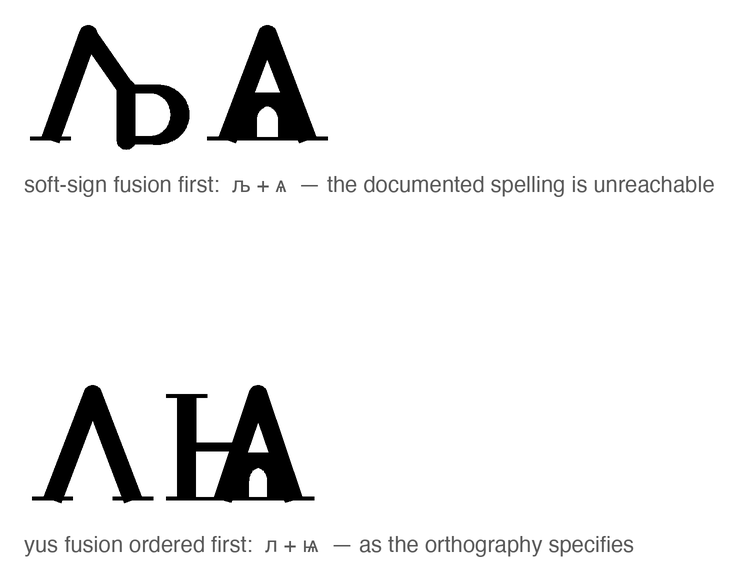
\includegraphics[width=0.61\linewidth]{figures/fig12_lookup_order.png}
\caption{Lookup order as orthographic law. Above: soft-sign fusion first — л+ь fuse, stranding the big yus; the spelling \cz{лѭ} cannot be typed. Below: the shipped order — yus fusion first.}\label{fig:order}
\end{figure}

\begin{figure}[ht]\centering
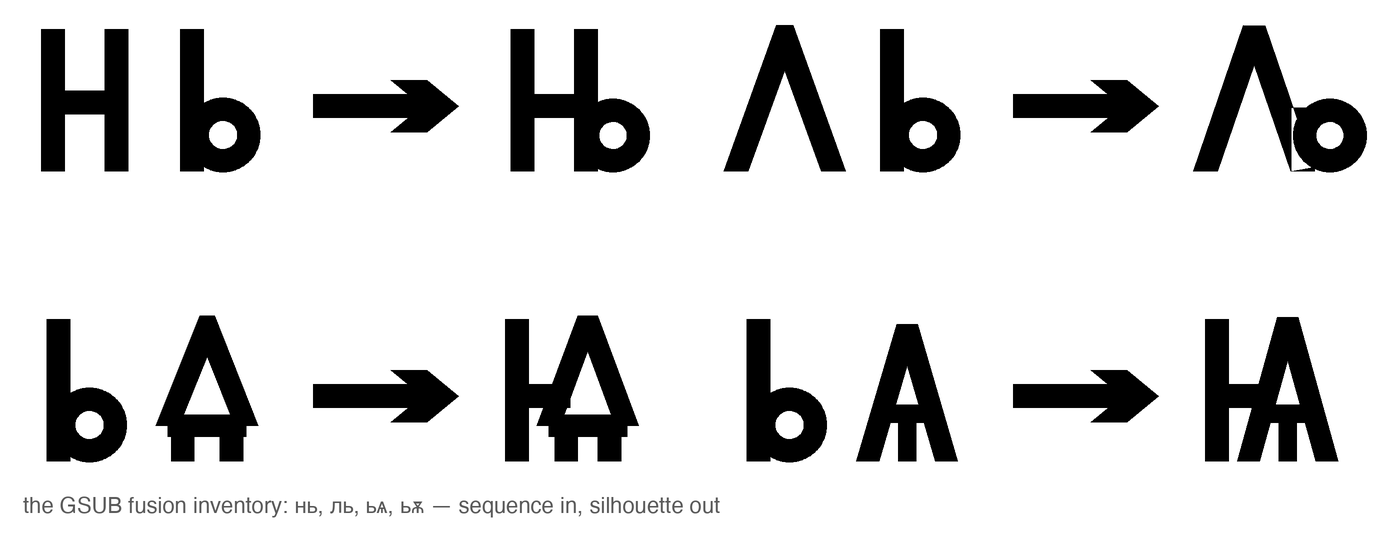
\includegraphics[width=1.00\linewidth]{figures/fig13_fusions.png}
\caption{The GSUB fusion inventory: \cz{нь} and \cz{ль} into fused forms; soft sign plus nasal into the iotated yuses. Sequence in, silhouette out; the components' separate identities do not survive, by design.}\label{fig:fusions}
\end{figure}

\begin{figure}[ht]\centering
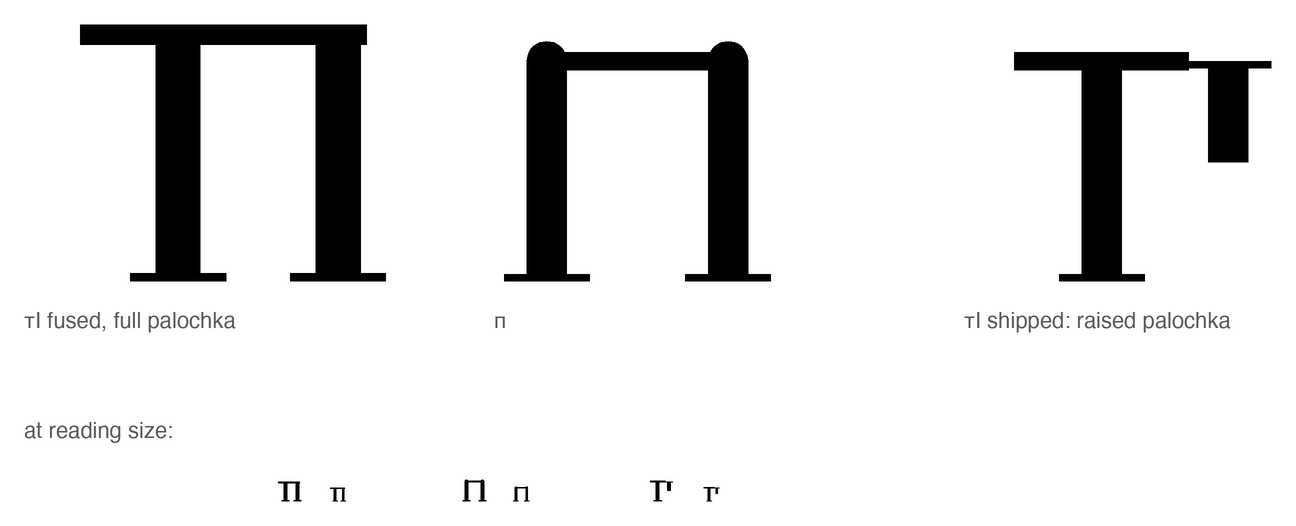
\includegraphics[width=1.00\linewidth]{figures/fig7_ligature.png}
\caption{The ejective ligature's silhouette rule. Left: \cz{тӀ} fused with a full-height palochka. Center: \cz{п} — at reading size (bottom row) the full-height fusion collapses into its frame. Right: the shipped fusion, palochka raised to the upper half, which survives smallness.}\label{fig:liga}
\end{figure}

\textbf{Mark law.} Every combining mark carries GPOS anchors computed per style from the built contours — the macron of \cz{а̄} attaches roughly 230 units lower than that of \cz{А̄}; the retroflex hook of \cz{т̢} lands on the letter's stem, not its visual center — so the specification's statement ``the hook attaches to the working stem'' is a checkable property of the artifact rather than a description of intent (Figure~\ref{fig:anchors}). Because anchors are computed from the contours each style actually built, the Inline's $\times$0.88 vertical compression is covered without any anchor-specific code.

\begin{figure}[ht]\centering
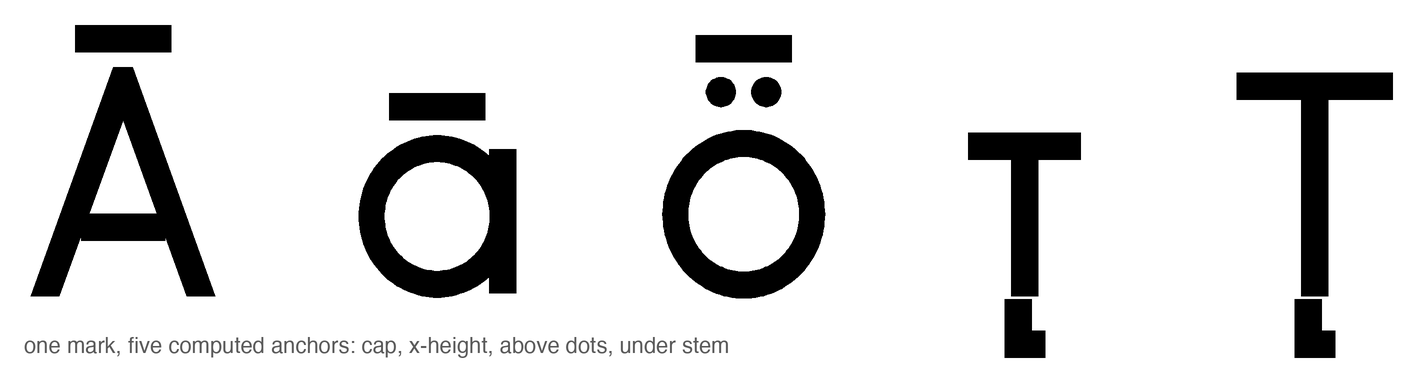
\includegraphics[width=1.00\linewidth]{figures/fig8_anchors.png}
\caption{One mark, many computed homes. The macron seats at cap height on \cz{А}, at x-height on \cz{а}, above the baked-in dots of \cz{ӧ}; the retroflex hook finds the stem of \cz{т} in either case. No anchor was placed by hand.}\label{fig:anchors}
\end{figure}

\textbf{Coverage law.} Unicode normalization composes \cz{е}+grave into precomposed \cz{ѐ} (U+0450) and \cz{и}+grave into \cz{ѝ} (U+045D); a font that lacks those codepoints watches browsers silently substitute a fallback face for exactly those letters, defeating the register that is the whole point. The character map therefore covers the NFC closure of every sequence the orthography can produce — 184 codepoints per family, including the citation punctuation — and the palochka ligatures accept the caseless \cz{Ӏ} (U+04C0) beside lowercase letters, because that is how Caucasian orthographies actually type it.

The test suite executes these laws through the deployment shaping stack (HarfBuzz; rasterization through FreeType): fusion-order assertions (\cz{льѧ} must shape to \cz{л}+\cz{ѩ}, never \cz{љ}+\cz{ѧ}), exact-sequence shaping checks for every documented fusion, mark-anchoring checks under the italic shear and the Inline compression, coverage parity across all four families, and the normalization-closure test, which NFC-normalizes every orthography-generable spelling and asserts no codepoint falls outside the cmap.

\section{At reading sizes}

Chuzhditsa is designed for \emph{embedded} settings — loanwords and names inside ordinary Cyrillic text, dictionary pronunciation fields, captions, pedagogy, and display — not for long-form running text. The evaluation targets that use: the face must keep its extension letters distinct, and their marks alive, at caption sizes inside someone else's paragraph. The boundary should be stated plainly: the evaluation is instrumented and proofed, not behavioral — no reading study with Cyrillic readers has been run, and the instrumentation certifies the absence of specific, named failure classes, not typographic quality.

The harness (\texttt{tools/eval\_smallsize.py}) renders glyph pairs through FreeType at fixed pixel sizes, thresholds ink at 50\%, and measures mark survival (ink pixels strictly above the base letter's topmost row) and confusable-pair contrast (symmetric difference of ink), worst-case across rasterization phases where noted. Table~\ref{tab:sizes} gives the 2b numbers; Figures \ref{fig:waterfall} and \ref{fig:confusables} show the rendered evidence, with small sizes magnified pixel-for-pixel rather than smoothed. The measured floors: \textbf{Grotesk and Serif hold a 12\,px floor; the 2b, 14; the Inline, 15.}

\begin{table}[ht]\centering\small
\begin{tabular}{rcccccccc}
\toprule
px & breve \cz{ў} & macron \cz{ӣ} & umlaut \cz{ӓ} & \cz{с}/\cz{ҫ} & \cz{з}/\cz{ҙ} & \cz{к}/\cz{қ} & \cz{е}/\cz{є} & \cz{о} counter R/B \\
\midrule
10 & 2 & 3 & 2 & 6 & 9 & 1 & 3 & open/open \\
12 & 2 & 4 & 2 & 6 & 1 & 5 & 5 & open/open \\
14 & 4 & 5 & 3 & 2 & 8 & 8 & 3 & open/open \\
18 & 7 & 6 & 5 & 19 & 10 & 3 & 12 & open/open \\
24 & 11 & 16 & 6 & 32 & 24 & 12 & 18 & open/open \\
\bottomrule
\end{tabular}
\caption{Instrumented small-size check of the shipped 2b binaries (Regular), FreeType rendering, 50\% ink threshold. Mark columns: ink pixels above the base letter's top. Pair columns: symmetric difference of ink in pixels. The 14\,px row is the floor row. The metric is comparative, not psychophysical: values below roughly 3--4 pixels are treated as suspect under visual inspection, and values need not rise monotonically with size, since rasterization and thresholding interact with grid phase.}
\label{tab:sizes}
\end{table}

The Inline's higher floor is arithmetic, not fragility, and belongs in the record because this manuscript's object language is set in it. At contrast 0.54 its horizontals are ${\approx}37/1000$\,em: at 10\,px that is 0.37\,px of geometric ink, which cannot clear a 50\% threshold at any rasterization phase. Measured phase-robustly, \cz{н}'s crossbar connects from 11\,px, the macron of \cz{ӣ} holds three pixels from 11\,px, and the \cz{к}/\cz{қ} hook contrast — the last probe to clear — is size-quantized at a single pixel through 14\,px and two or more from 15. Scoped honestly: in print the Inline is safe (at 150\,dpi its floor is under 8\,pt); at 96\,dpi on screen it is dependable from 12\,pt and marginal at 11. The near-monoline cuts' lower floors quantify the monoline advantage — no hairlines to drop out — and the family carries its own counterexample in the cut that trades that advantage for color match.

\begin{figure}[ht]\centering
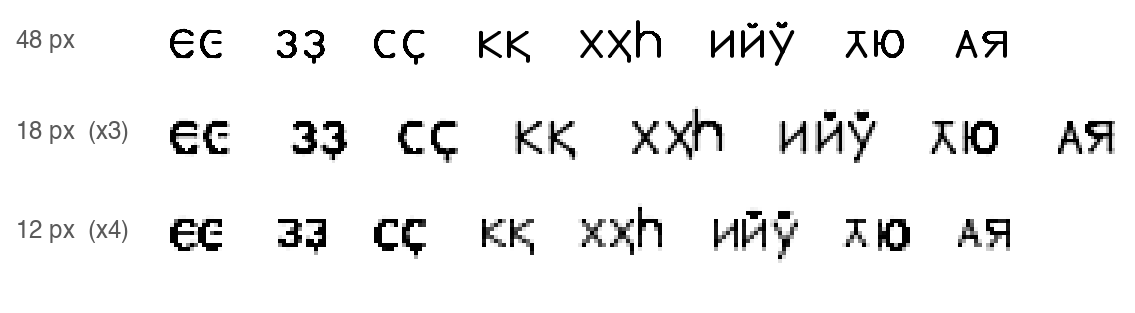
\includegraphics[width=0.9\linewidth]{figures/fig18_confusables.png}
\caption{Confusable pairs at reading sizes, FreeType rendering: \cz{е}/\cz{є}, \cz{з}/\cz{ҙ}, \cz{с}/\cz{ҫ}, \cz{к}/\cz{қ}, \cz{х}/\cz{ҳ}/\cz{һ}, \cz{и}/\cz{й}/\cz{ў}, \cz{ѫ}/\cz{ю}, \cz{ѧ}/\cz{я}. The 18 and 12 pixel rows are nearest-neighbor magnifications of the actual rasters — what the renderer produced, not what the vector promises.}\label{fig:confusables}
\end{figure}

\begin{figure}[ht]\centering
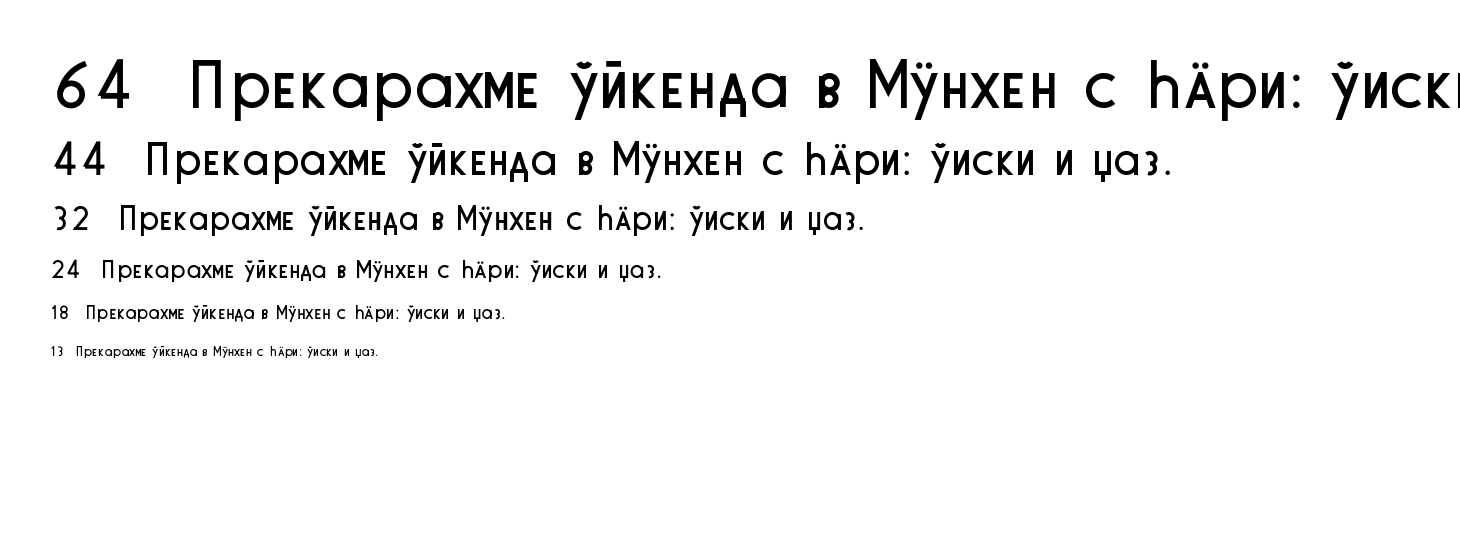
\includegraphics[width=\linewidth]{figures/fig16_waterfall.png}
\caption{Waterfall, FreeType rendering, 64 down to 13 pixels. The marks — breve, macron, umlaut, hooks — are the stress test: a citation register that loses its diacritics at caption sizes has lost its phonology.}\label{fig:waterfall}
\end{figure}

\section{Pipeline and reproducibility}

The builder is $\sim$800 lines of Python on \texttt{fontTools}. Glyph skeletons are declared as the centerline primitives of \S2; the character map is generated from a single codepoint table including the NFC closure; GSUB and GPOS are emitted as AFDKO feature source and compiled by \texttt{feaLib}; TrueType and CFF are cut from identical contours (\texttt{TTGlyphPen}, \texttt{T2CharStringPen}). The sixteen styles are not interpolated but \emph{re-evaluated}: the same skeletons under different parameter sheets, which makes structural agreement across styles a consequence of the source model rather than a per-glyph discipline. The build is byte-reproducible — timestamps are pinned via \texttt{SOURCE\_DATE\_EPOCH}, set in-script and overridable in the environment — so identical source yields identical binaries, and any claimed property of the shipped fonts can be re-derived from the repository at the commit that shipped them.

Two implementation notes are recorded for the next implementer. First, outline hygiene: overlapping contours with mixed orientation cancel under nonzero winding just as surely as folds render white under even-odd — orient before you overlap, or union before you emit; this engine unions. Second, the legacy \texttt{kern} table is dead in CFF-flavored fonts: HarfBuzz ignores it there, and pair kerning that tests correctly in a parser can still be a no-op in every browser. GPOS or nothing.

\section{Limitations}\label{sec:limits}

Dense polygon outlines trade analytic exactness for simplicity; a Bézier or variable-font export remains unbuilt (weight, slant, and contrast are already parameters, so a variable export is the natural successor). There is no language-specific localized-forms layer (Bulgarian-form alternates would be the natural first set) and no mark-to-mark positioning, which caps stacked prosody. The tangent-angle function is a texture correction, not a contrast \emph{axis}: it has no pen angle, no translation model, and no ambition beyond ten percent at the base — a true expansion-model contrast would promote the engine from eight hundred lines to a research project, precisely the slope on which METAFONT's practical reputation perished (Southall, 1985). The italic is a corrected oblique, not a cursive: shearing centerlines before expansion yields a mathematically coherent slanted construction, not a resolved italic design in the cultural sense; a true italic would need new skeletons, which is to say, new writing. The register's visual layer is fragile under font fallback (\S1's encoding distinction), behavior in office suites and mobile rendering stacks is untested, and every legibility claim here is instrumented or proofed, none behavioral. Everything reported is a transparent case study of one constrained design grammar in a deliberately small engine; no claim is made that the findings transfer to production workflows with true curves, hinting, or interpolation across masters.

\section{Conclusion}

The contribution this paper shares with its companion is vertical integration: a phonological distinction is traceable without a gap through a graphemic operation, a Unicode sequence, a glyph construction, an OpenType behavior, and a rendered artifact — and each level is testable at its own altitude. The reusable contribution is not the Chuzhditsa aesthetic: it is the demonstration that a small stroke grammar, an explicit optical canon, and a shaping-test harness suffice to produce and verify a coherent multi-style script-extension family — a recipe portable to any register, any script, any design language willing to state its rules. A caution travels with the recipe: the failure classes the rules of \S\ref{sec:rules} guard against (naïve terminals, cancelling overlaps, clogging arcs, unadapted bold fitting) are intrinsic to centerline expansion, but the particular thresholds, clamps, and class structures are this design language's choices, and another grammar would choose differently. The construction vindicates a modest form of Knuth's programme — parameters within one design language, never across all of them — and confirms an old suspicion of the drawing office: that most of what reads as beauty in geometric type is a ledger of small, principled lies to Euclid, and that the ledger, at last, can be source code.

\begin{thebibliography}{99}
\bibitem{bigelow} Bigelow, C., \& Holmes, K. (1993). The design of a Unicode font. \emph{Electronic Publishing}, \emph{6}(3), 289--305.
\bibitem{bringhurst} Bringhurst, R. (2004). \emph{The elements of typographic style} (3rd ed.). Hartley \& Marks.
\bibitem{burke} Burke, C. (1998). \emph{Paul Renner: The art of typography}. Hyphen Press.
\bibitem{hofstadter} Hofstadter, D. R. (1982). Metafont, metamathematics, and metaphysics: Comments on Donald Knuth's article ``The concept of a meta-font''. \emph{Visible Language}, \emph{16}(4), 309--338.
\bibitem{johnston} Johnston, E. (1906). \emph{Writing \& illuminating, \& lettering}. John Hogg.
\bibitem{knuth82} Knuth, D. E. (1982). The concept of a meta-font. \emph{Visible Language}, \emph{16}(1), 3--27.
\bibitem{noordzij} Noordzij, G. (2005). \emph{The stroke: Theory of writing}. Hyphen Press.
\bibitem{smeijers} Smeijers, F. (1996). \emph{Counterpunch: Making type in the sixteenth century, designing typefaces now}. Hyphen Press.
\bibitem{southall} Southall, R. (1985). \emph{Designing new typefaces with Metafont} (Report No.\ STAN-CS-85-1074). Stanford University, Department of Computer Science.
\bibitem{tracy} Tracy, W. (1986). \emph{Letters of credit: A view of type design}. Gordon Fraser.
\bibitem{yonchev} Yonchev, V., \& Yoncheva, O. (1982). \emph{Древен и съвременен български шрифт} [Ancient and modern Bulgarian type]. Balgarski hudozhnik.
\bibitem{zhukov} Zhukov, M. (1996). The peculiarities of Cyrillic letterforms: Design variation and correlation in Russian typefaces. \emph{Typography Papers}, \emph{1}.
\end{thebibliography}

\end{document}
